\providecommand\ExamFontPath{../../../字体/}
\documentclass[fontset=exam]{exam-zh}
\usepackage{longtable,booktabs,array,calc,multirow,fvextra}
\usepackage[normalem]{ulem}
\providecommand{\hl}[1]{#1}
\providecommand{\ul}[1]{\uline{#1}}
\DefineVerbatimEnvironment{verbatim}{Verbatim}{breaklines=true,fontsize=\small}
\providecommand{\tightlist}{\setlength{\itemsep}{0pt}\setlength{\parskip}{0pt}}
\newcommand{\pandocbounded}[1]{#1}
\setlength{\emergencystretch}{3em}
\setlength{\tabcolsep}{2pt}
\examsetup{page/size=a4paper}
\title{厦门大学 2021 年 期末考试 A 卷}
\subject[4em]{概率统计}
\begin{document}
\maketitle
\fancyfoot[C]{第 \thepage 页（共 \pageref*{LastPage} 页）}
\pdfbookmark[1]{一、选择题（在各小题四个备选答案中选出一个正确答案，填在题末的括号中，本大题共6个小题，每小题3分，总计18分）}{section1}

\par\medskip{\heiti

一、选择题（在各小题四个备选答案中选出一个正确答案，填在题末的括号中，本大题共 6 个小题，每小题 3 分，总计 18 分）

\par}\smallskip

\begin{enumerate}
\def\labelenumi{\arabic{enumi}.}
\item
  已知\(X\sim1/t(n)\)，则以下选项正确的是（）
\end{enumerate}

\begin{quote}
A \(X^2\sim F(n,1)\) B \(X^2\sim F(n,n)\)

C \(X^2\sim F(1,n-1)\) D \(X^2\sim F(1,n)\)
\end{quote}

\begin{enumerate}
\def\labelenumi{\arabic{enumi}.}
\setcounter{enumi}{1}
\item
  设\(X_1,X_2,\ldots,X_n\)是取自总体\(X\)的一个随机样本，\(E(X)=\mu,D(X)=\sigma^2\), \(\widehat\theta^2=C\sum_{i=1}^{n-1}(X_{i+1}-X_i)^2\)为\(\sigma^2\)的无偏估计，则\(C=\)（）
\end{enumerate}

\begin{quote}
A．\(1/n\) B. \(1/(n-1)\)

C. \(1/2(n-1)\) D. \(1/(n-2)\)
\end{quote}

\begin{enumerate}
\def\labelenumi{\arabic{enumi}.}
\setcounter{enumi}{2}
\item
  对正态总体的数学期望\(\mu\)进行假设检验，如果在显著性水平 0.05 下接受\(H_0:\mu=\mu_0\), 那么在显著性水平 0.01 下,下列结论中正确的是 ( )
\end{enumerate}

\begin{quote}
A 必须接受\(H_0\) B 可能接受,也可能拒绝\(H_0\)

C 必定拒绝\(H_0\) D 不接受,也不拒绝\(H_0\)
\end{quote}

\begin{enumerate}
\def\labelenumi{\arabic{enumi}.}
\setcounter{enumi}{3}
\item
  设\(X_1,X_2,\ldots,X_n\)为来自正态总体\(N(\mu,\sigma^2)\)的一个简单随机样本, 若进行假设检验,当\underline{\hspace{2cm}}时, 检验使用的统计量是\(t=\frac{\overline X-\mu_0}{S/\sqrt n}\).
\end{enumerate}

\begin{quote}
A \(\mu\)未知, 检验\(\sigma^2=\sigma_0^2\) B \(\mu\)已知, 检验\(\sigma^2=\sigma_0^2\)

C \(\sigma^2\)未知, 检验\(\mu=\mu_0\) D \(\sigma^2\)已知, 检验\(\mu=\mu_0\)
\end{quote}

\begin{enumerate}
\def\labelenumi{\arabic{enumi}.}
\setcounter{enumi}{4}
\item
  设\(X_1,X_2,\ldots,X_n\)为来自正态总体\(N(\mu,\sigma^2)\)的一个简单随机样本, 按给定的显著性水平\(\alpha\)检验\(H_0:\mu=\mu_0\)(已知), \(H_1:\mu\ne\mu_0\)时, 判断是否接受\(H_0\)与 ( ) 有关.
\end{enumerate}

\begin{quote}
A 样本值,显著性水平\(\alpha\) B 样本值,样本容量\(n\)

C 样本容量\(n\),显著性水平\(\alpha\) D 样本值,样本容量\(n\),显著性水平\(\alpha\)
\end{quote}

\begin{enumerate}
\def\labelenumi{\arabic{enumi}.}
\setcounter{enumi}{5}
\item
  设随机变量\(X_1,X_2,\ldots,X_n\)相互独立分布， \(S_n=X_1+X_2+\cdots+X_n\)，根据中心极限定理，当\(n\)充分大，\(S_n\)近似服从正态分布，只要\(X_1,X_2,\ldots,X_n\)（ ）
\end{enumerate}

\begin{quote}
A 有相同的数学期望 B 有相同的方差

C 服从同一指数分布 D 服从同一离散型分布
\end{quote}

\pdfbookmark[1]{二、填空题（本大题共6小题，每小题3分，总计18分）}{section14}

\par\medskip{\heiti

二、填空题（本大题共 6 小题，每小题 3 分，总计 18 分）

\par}\smallskip

\begin{enumerate}
\def\labelenumi{\arabic{enumi}.}
\item
  设\(X\sim N(\mu,0.3^2)\)，容量\(n=9\)，均值\(\overline X=5\)，则未知参数\(\mu\)的置信度为 0.95 的置信区间是\underline{\hspace{2cm}}。（查表\(z_{0.025}=1.96,z_{0.05}=1.64\)）
\item
  设\(X_1,X_2,\ldots,X_n\)为来自正态总体\(N(\mu,\sigma^2)\)的一个简单随机样本, 其中参数\(\mu\)和\(\sigma^2\)均未知, 记\(\overline X=\frac1n\sum_{i=1}^nX_i\), \(Q^2=\sum_{i=1}^n(X_i-\overline X)^2\), 则假设\(H_0:\mu=0\)的\emph{t}检验使用的统计量是\underline{\hspace{2cm}}。 (用\(\overline X\)和\(Q\)表示)
\item
  设在显著性检验中, 若要使犯两类错误的概率同时变小, 则只有\underline{\hspace{2cm}}
\item
  设总体\(X\sim N(\mu,\sigma^2)\),\(\mu,\sigma^2\)为未知参数, 从\(X\)中抽取的容量为\(n\)的样本均值记为\(\overline X\), 现在要检验假设\(H_0:\mu=\mu_0\), \(H_1:\mu\ne\mu_0\)时, 则应该选择的统计量是\underline{\hspace{2cm}}; 当\(H_0:\mu=\mu_0\)成立时,该统计量服从\underline{\hspace{2cm}}分布.
\item
  设在总体\(X\sim N(\mu,\sigma^2)\)中抽得一容量为 21 的样本，这里\(\mu,\sigma^2\)均未知，则\(D(S^2)\)=\underline{\hspace{2cm}}
\item
  设\(X\sim N(\mu_X,\sigma_X^2)\)，\(Y\sim N(\mu_Y,\sigma_Y^2)\)，且\(X\)与\(Y\)相互独立，设\(X_1,X_2,\ldots,X_m\)为来自总体\(X\)的一个样本，\(Y_1,Y_2,\ldots,Y_n\)为来自总体\(Y\)的一个样本，\(S_X^2\)和\(S_Y^2\)分别是其无偏样本方差，则\[\frac{S_X^2/\sigma_X^2}{S_Y^2/\sigma_Y^2}\]服从的分布是\underline{\hspace{2cm}}。
\end{enumerate}

\pdfbookmark[1]{三、（8分）设某车间有200台车床相互独立地工作着，若因换料、检修等原因，每台车床的开工各为0.6，开工时耗电各位1千瓦}{section16}

三、（8 分）设某车间有 200 台车床相互独立地工作着，若因换料、检修等原因，每台车床的开工各为 0.6，开工时耗电各位 1 千瓦，问供电所至少要供给这个车间多少千瓦电，才能以 99.9\%的概率保证这个车间不会因供电不足而影响生产？

\pdfbookmark[1]{四、（8分）设抽取简单随机样本，样本均值，求.}{section17}

四、（8 分）设\(X\sim N(\mu,\sigma^2)\)抽取简单随机样本\(X_1,X_2,\ldots,X_{2n}\ (n\geq2)\)，样本均值\(\overline X=\frac1{2n}\sum_{i=1}^{2n}X_i\)，\(Y=\sum_{i=1}^n(X_i+X_{i+n}-2\overline X)^2\)求\(E(Y)\).

\pdfbookmark[1]{五、（14分）设随机变量的密度函数为 ，求的极大似然估计。}{section18}

五、（14 分）设随机变量\(X\)的密度函数为 \(f(x)=\begin{cases}(\lambda+1)x^2,&0<x<1,\\0,&else\end{cases}\)，求\(\lambda\)的极大似然估计。

\pdfbookmark[1]{六、（14分）某矿地出产的矿石含有某种少量元素，其含量服从正态分布。抽取12个样本进行调查，算得，求的置信区间。（）}{section19}

六、（14 分）某矿地出产的矿石含有某种少量元素，其含量服从正态分布。抽取 12 个样本进行调查，算得\(S=0.2\)，求\(\sigma\)的置信区间。（\(\alpha=0.1,\chi^2_{\alpha/2}(11)=19.68,\chi^2_{1-\alpha/2}(11)=4.57\)）

\pdfbookmark[1]{七、（10分）设某电子元件使用寿命(单位: 小时)服从正态分布. 从该种电子元件中随机抽取25个进行测试, 测得平均使用}{section20}

七、（10 分）设某电子元件使用寿命(单位: 小时)服从正态分布\(N(\mu,80^2)\). 从该种电子元件中随机抽取 25 个进行测试, 测得平均使用寿命为 968 小时, 标准差不变. 问: 在显著性水平\(\alpha=0.005\)条件下, 是否可以认为该种电子元件平均使用寿命为 1000 小时?

\pdfbookmark[1]{八、（10分）设已知随机变量相互独立，且其均值一致有界，即是存在常数AB使得，证明服从大数定律。}{section21}

八、（10 分）设已知随机变量\(X_1,X_2,\ldots,X_n\)相互独立，且其均值一致有界，即是存在常数 AB 使得\(E(X_i)<A,D(X_i)<B\)，证明\(X_1,X_2,\ldots,X_n\)服从大数定律。

附表： \(\Phi(x) = {\int_{- \infty}^{x}{\frac{1}{\sqrt{2\pi}}e^{- \frac{t^{2}}{2}}dt}}\)

\begin{longtable}[]{@{}
  >{\centering\arraybackslash}p{(\linewidth - 20\tabcolsep) * \real{0.0563}}
  >{\centering\arraybackslash}p{(\linewidth - 20\tabcolsep) * \real{0.0944}}
  >{\centering\arraybackslash}p{(\linewidth - 20\tabcolsep) * \real{0.0944}}
  >{\centering\arraybackslash}p{(\linewidth - 20\tabcolsep) * \real{0.0944}}
  >{\centering\arraybackslash}p{(\linewidth - 20\tabcolsep) * \real{0.0944}}
  >{\centering\arraybackslash}p{(\linewidth - 20\tabcolsep) * \real{0.0944}}
  >{\centering\arraybackslash}p{(\linewidth - 20\tabcolsep) * \real{0.0944}}
  >{\centering\arraybackslash}p{(\linewidth - 20\tabcolsep) * \real{0.0944}}
  >{\centering\arraybackslash}p{(\linewidth - 20\tabcolsep) * \real{0.0944}}
  >{\centering\arraybackslash}p{(\linewidth - 20\tabcolsep) * \real{0.0944}}
  >{\centering\arraybackslash}p{(\linewidth - 20\tabcolsep) * \real{0.0940}}@{}}
\toprule\noalign{}
\endhead
\bottomrule\noalign{}
\endlastfoot
\emph{x} & 0 & 0.01 & 0.02 & 0.03 & 0.04 & 0.05 & 0.06 & 0.07 & 0.08 & 0.09 \\
1 & 0.841 3 & 0.843 8 & 0.846 1 & 0.848 5 & 0.850 8 & 0.853 1 & 0.855 4 & 0.857 7 & 0.859 9 & 0.862 1 \\
1.1 & 0.864 3 & 0.866 5 & 0.868 6 & 0.870 8 & 0.872 9 & 0.874 9 & 0.877 0 & 0.879 0 & 0.881 0 & 0.883 0 \\
1.2 & 0.884 9 & 0.886 9 & 0.888 8 & 0.890 7 & 0.892 5 & 0.894 4 & 0.896 2 & 0.898 0 & 0.899 7 & 0.901 5 \\
1.3 & 0.903 2 & 0.904 9 & 0.906 6 & 0.908 2 & 0.909 9 & 0.911 5 & 0.913 1 & 0.914 7 & 0.916 2 & 0.917 7 \\
1.4 & 0.919 2 & 0.920 7 & 0.922 2 & 0.923 6 & 0.925 1 & 0.926 5 & 0.927 9 & 0.929 2 & 0.930 6 & 0.931 9 \\
& & & & & & & & & & \\
1.5 & 0.933 2 & 0.934 5 & 0.935 7 & 0.937 0 & 0.938 2 & 0.939 4 & 0.940 6 & 0.941 8 & 0.943 0 & 0.944 1 \\
1.6 & 0.945 2 & 0.946 3 & 0.947 4 & 0.948 4 & 0.949 5 & 0.950 5 & 0.951 5 & 0.952 5 & 0.953 5 & 0.953 5 \\
1.7 & 0.955 4 & 0.956 4 & 0.957 3 & 0.958 2 & 0.959 1 & 0.959 9 & 0.960 8 & 0.961 6 & 0.962 5 & 0.963 3 \\
1.8 & 0.964 1 & 0.964 8 & 0.965 6 & 0.966 4 & 0.967 2 & 0.967 8 & 0.968 6 & 0.969 3 & 0.970 0 & 0.970 6 \\
1.9 & 0.971 3 & 0.971 9 & 0.972 6 & 0.973 2 & 0.973 8 & 0.974 4 & 0.975 0 & 0.975 6 & 0.976 2 & 0.976 7 \\
& & & & & & & & & & \\
2 & 0.977 2 & 0.977 8 & 0.978 3 & 0.978 8 & 0.979 3 & 0.979 8 & 0.980 3 & 0.980 8 & 0.981 2 & 0.981 7 \\
2.1 & 0.982 1 & 0.982 6 & 0.983 0 & 0.983 4 & 0.983 8 & 0.984 2 & 0.984 6 & 0.985 0 & 0.985 4 & 0.985 7 \\
2.2 & 0.986 1 & 0.986 4 & 0.986 8 & 0.987 1 & 0.987 4 & 0.987 8 & 0.988 1 & 0.988 4 & 0.988 7 & 0.989 0 \\
2.3 & 0.989 3 & 0.989 6 & 0.989 8 & 0.990 1 & 0.990 4 & 0.990 6 & 0.990 9 & 0.991 1 & 0.991 3 & 0.991 6 \\
2.4 & 0.991 8 & 0.992 0 & 0.992 2 & 0.992 5 & 0.992 7 & 0.992 9 & 0.993 1 & 0.993 2 & 0.993 4 & 0.993 6 \\
\end{longtable}

\par\medskip{\centering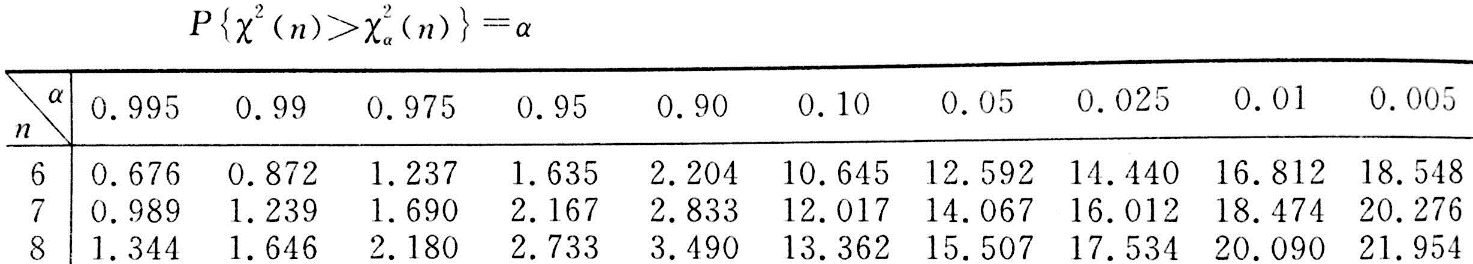
\includegraphics[width=15cm]{figures/image74.png}\par}\medskip \par\medskip{\centering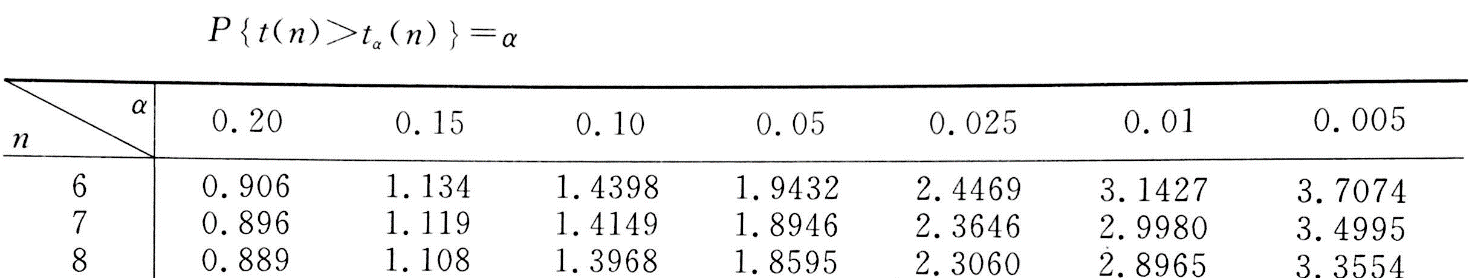
\includegraphics[width=15cm]{figures/image75.png}\par}\medskip

\end{document}
